\chapter{Asking Dubai Moguls How They Got Rich!}

This chapter follows a School of Hard Knocks interview, curated by LazyingArt LLC, and it should be read as a sequence of worked business motifs rather than as a single continuous theory announced all at once. We begin with spectacle, but the lecture quickly turns that spectacle into method: sales arithmetic, hardship thresholds, rapid capital formation, non-transactional networking, scalable technology, and finally a stage rule for concentration and diversification.

\section{Cold Open: Dubai, Scale, and the Teaser Splice}

The lecture opens by spending surprise before explanation. We hear fragments of later claims: a Lamborghini, a blockchain company, annual figures ranging from the low eight figures to one hundred million dollars, the phrase ``billion dollar company,'' and a net-worth-like number near three hundred million dollars. These lines do not yet form one coherent case. They function as a splice, a promise that the lecture will not merely discuss wealth in the abstract.

Only after that splice does the host reset the frame. We are in Dubai, and the city is treated as a field site in which visible luxury is not the argument but the bait. The real work of the lecture is to move from the object to the mechanism: what industry, what sequence of choices, what cash discipline, what communication style, what timing, and what form of capital allocation lie behind the visible result.

It is useful to register the opening numbers, but useful in the right way. They are not yet equations in a single system. They are markers of scale that the later sections will unpack one by one.

\section{From Rent Pressure to the Arithmetic of Sales}

The first sustained case is the Lamborghini owner in finance. The movement is very deliberate. First we are given duration and scale; only then are we taken backward into scarcity:
\begin{align}
t_{\text{James}} &\approx 8\ \text{years}, \\
Y_{\text{James}}^{\text{turnover}} &\approx \$12\,\text{million}, \\
R_{\text{rent}} &\approx \$1{,}300.
\end{align}
The lecture does not leave the eight-figure turnover floating in the air. It binds it to a concrete threshold: there was a time when rent at roughly \$1{,}300 was not payable, and the family had to sell wedding jewelry in order to survive. That is the lecture's first serious structural move. Wealth is not merely displayed; it is measured against a previous bottleneck.

The next move is psychological, but it is not merely sentimental. The speaker says the turning point was inward: not finishing school, being the black sheep, and cultivating the desire to prove that a degree was not the only route to large-scale success. Then the lecture narrows again from attitude to operating control. ``Full control over the money'' means knowing where money comes from, where it goes, and refusing to surrender that visibility to operators who may later control the business more than the founder does.

At this point the host asks the right follow-up question. If the business is now large, how does one actually produce yeses in the field rather than merely wishing for them?

\subsection{Question \& Answer}

The question is simple: what does it mean to get to yes faster? The answer is not a polished theory of persuasion. It is a very practical sequence taken from door-to-door sales:
\begin{equation}
N_{\text{doors}} = 100,
\qquad
n_{\text{ask}} \approx 4\text{--}5.
\end{equation}
The point is not that one giant pitch suddenly works. The point is that repeated attempts produce information, and information lets us improve the next attempt. The lecture's local model can be written schematically as
\begin{equation}
\text{yes} \to \text{yes} \to \text{yes} \to \text{ask},
\qquad
P(\text{yes on ask }4\text{ or }5)\ \text{rises}.
\end{equation}
This is not offered as a statistical law. It is offered as a field rule: accumulate small agreements before making the real request.

A worked example is given directly in the interview:
\begin{align}
Q_1 &: \text{Are you in Dubai?} & A_1 &= \text{yes}, \\
Q_2 &: \text{Do you like the weather here?} & A_2 &= \text{yes}, \\
Q_3 &: \text{Do you like the vibe here?} & A_3 &= \text{yes}, \\
Q_4 &: \text{Would you like to own property here one day?} & A_4 &= \text{soft yes}.
\end{align}
The lecture's claim is that once the first three affirmations have been secured, the fourth question can be pushed from hesitation toward agreement. The host compresses the doctrine well: amateurs tell, pros ask.

\begin{figure}[h]
\centering
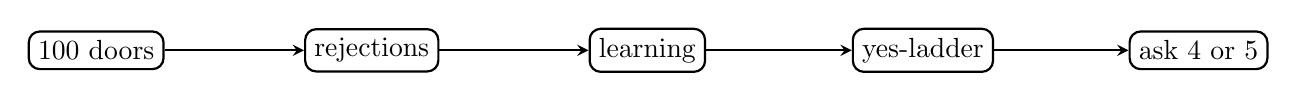
\begin{tikzpicture}[>=stealth, thick]
\node[draw, rectangle, rounded corners] (a) at (0,0) {\(100\) doors};
\node[draw, rectangle, rounded corners] (b) at (3.5,0) {rejections};
\node[draw, rectangle, rounded corners] (c) at (7,0) {learning};
\node[draw, rectangle, rounded corners] (d) at (10.5,0) {yes-ladder};
\node[draw, rectangle, rounded corners] (e) at (14,0) {ask \(4\) or \(5\)};
\draw[->] (a) -- (b);
\draw[->] (b) -- (c);
\draw[->] (c) -- (d);
\draw[->] (d) -- (e);
\end{tikzpicture}
\caption{Transcript-based reconstruction of the first speaker's sales mechanism.}
\end{figure}

The lecture then broadens from sales to austerity. During the broke phase the speaker cut subscriptions, delayed rewards, and preferred saving and investing to immediate convenience. The text around tiny subscription costs is garbled in the transcript, so we should not invent a neat budget identity that the lecture does not actually provide. But the structural claim is clear enough: sacrifice first, reward later, and let execution dominate commentary. An idea should not be judged by spectators with no business experience; it should be judged by whether it is actually built.

\section{Fast Scale, Timing, and the Web3 Friction Thesis}

The second major case changes the scale and the time horizon at once. Now the lecture is not about moving from hardship to a twelve-million-dollar turnover. It is about the speed with which a blockchain company can become a unicorn:
\begin{align}
\Delta t_{\text{raise}} &\approx 11\ \text{months}, \\
M_{\text{raised}} &> \$100\,\text{million}, \\
V_{\text{company}} &\approx \$1.5\,\text{billion}.
\end{align}
This is the lecture's cleanest capital-formation example. The company is said to have started in April 2021, raised more than one hundred million dollars within roughly eleven months, and reached a valuation of about one and a half billion dollars in that same window.

We may even compute the rough average pace implied by the transcript:
\begin{equation}
\frac{M_{\text{raised}}}{\Delta t_{\text{raise}}}
\gtrsim
\frac{\$100\,\text{million}}{11\ \text{months}}
\approx
\$9.1\,\text{million per month}.
\end{equation}
The lecture itself does not present the ratio this way, but the arithmetic helps us see what ``fast'' means in operational terms.

\subsection{Question \& Answer}

Can one get rich quickly in such a world? The answer given here is precise in one sense and vague in another. It is precise about structure and vague about prediction. The structure is this: what matters is not merely being in the right location but choosing the right expanding industry at the right historical moment. The lecture compresses that logic into a historical ladder,
\begin{equation}
1990\text{s} \to \text{internet},
\qquad
2010\text{s} \to \text{social media},
\qquad
2020\text{s} \to \text{AI / blockchain / Web3}.
\end{equation}
So ``rich quick'' is not really framed as magic. It is framed as temporal matching: effort attached to an industry whose curve is still rising.

From that point the speaker turns the argument into a friction story about crypto. Banks, in this telling, make money on our money. Crypto, by contrast, is described as a system in which our own money compounds more directly:
\begin{align}
c_{\text{crypto}}(\$10\,\text{million}) &\approx \$1, \\
T_{\text{crypto exit}}(\$15\,\text{million}) &\approx 1\ \text{minute}.
\end{align}
We should state these carefully. They are not universal theorems. They are strong speaker claims, deployed rhetorically to contrast crypto transfer friction and real-estate illiquidity.

The speaker then adds a class-motion thesis: Web3 is presented as the place where poor can become middle class, middle class can become upper middle class, and upper middle class can become rich. The transcript should preserve that claim, but preserve it as doctrine, not as settled law. The lecture is most rigorous here when it speaks about timing and liquidity, not when it predicts the entire future of class mobility.

A sponsor block interrupts the momentum at exactly this point. The only conceptual residue worth carrying forward is the host's remark that rapid fundraising depends not only on industry selection but on communication quality. That observation is consistent with the lecture's broader insistence that language is itself a commercial instrument.

\section{Human Capital, Non-Transactional Contact, and Collision Hours}

After the interruption the lecture changes register. We move from blockchain speed to human method. A venture-capital and tech operator, who says he has been broke many times, supplies the most useful doctrine in the middle of the chapter: do not approach the wealthy transactionally. We are told not to talk about work first, not to treat the interaction as a grab for advantage, and not to mistake an outcome-seeking conversation for a real relationship.

The simplest reconstruction of the mechanism is
\begin{equation}
\text{human conversation}
\to
\text{shared affinity}
\to
\text{trust}
\to
\text{business opportunity}.
\end{equation}
This is again not a theorem. It is an operating sequence. The lecture insists that some of the best businesses do not begin with a business pitch at all. They begin with two people discovering that they share a setting, an event, a taste, or a value.

\subsection{Question \& Answer}

Why should business begin this way? Because, in the speaker's account, people usually ruin the interaction by entering with a desired outcome already in mind. If the immediate aim is extraction, the relationship never becomes human. If the relationship becomes human, then business can arrive later as a consequence rather than as a demand.

At precisely this point the lecture sharpens the claim by shifting from relationship to execution. It gives a benchmark:
\begin{equation}
S_{\text{Snuggie}} \approx \$100\,\text{million}.
\end{equation}
A blanket with sleeves is presented as a bad idea that was executed well, and from this the speaker derives the larger comparative principle
\begin{equation}
\text{bad idea executed well}
\;>\;
\text{great idea executed poorly}.
\end{equation}
This is one of the cleanest inequalities in the lecture. It rescues us from the habit of overvaluing concept purity and undervaluing the machinery of delivery.

The lecture then moves one step further. The speaker says he was originally a computer science graduate, more at home behind a screen than in direct social contact. But that is not enough. One must learn to speak. One must learn to meet people. One must create the occasions in which business can emerge. This is where Tony Hsieh's language of ``Collision Hours'' becomes important. We do not wait passively for high-value interactions; we construct environments in which they become likely.

\section{Scale, Go-to-Market, and the Five-Year Horizon}

From relationships the lecture returns to scale. The question is now explicit: how does one move from seven figures to eight? The answer begins with the architecture of the product itself. Tech is privileged because it scales without the physical bottlenecks that accompany ordinary goods. The lecture's logic can be summarized as
\begin{equation}
MC_{\text{digital}} \ll MC_{\text{physical}},
\qquad
\text{go-to-market reach} \to \text{global market}.
\end{equation}
When we produce software rather than a physical object, the next unit is not burdened by the same material cost. Then the bottleneck shifts from production to distribution. The question becomes: can we find the right users, build the right channel, and place the product before a market that is no longer local but global?

The lecture is careful not to stop there. Once scale has been described in present terms, the speaker asks how we choose the right sector before it becomes obvious to everyone else.

\subsection{Question \& Answer}

How do we choose a sector before the market has fully arrived? The lecture answers by refusing presentism. We are told to look five years forward, to imagine the world that is coming, and then to build for that world now:
\begin{equation}
\text{build at } t
\text{ for the world at } t+5.
\end{equation}
This is the most openly speculative but also the most structurally useful rule in the chapter. It is not merely ``follow AI'' or ``follow Web3.'' It is: decide what the future state demands, then occupy the enabling layer before that future is ordinary.

The lecture gives several examples of what such enabling layers might be: AI, automation, battery optimization, machine production, synthetic data, and even AI-avatar content systems. The point is not that all of these will win. The point is that one should build around the periphery that the coming system requires. At the same time, the lecture inserts a corrective. The most profitable business in the speaker's current portfolio is said to be mortgage technology, a reminder that boring businesses can be commercially superior to glamorous ones.

\section{The Final Stage Rule: Concentrate, Then Diversify}

The final Rolls-Royce and blockchain case provides a different kind of closure. We are again shown large numbers, but now the purpose is not merely to shock. It is to state a stage rule:
\begin{align}
Y_{\text{personal,last year}} &\approx \$100\,\text{million}, \\
W_{\text{net}} &\approx \$300\,\text{million}.
\end{align}
The host mishears one line as one hundred billion dollars, but the context clearly indicates one hundred million. That is large enough. The more important doctrine is what follows. When one has no money, one must go all in on the idea. Once money exists, one must become balanced:
\begin{equation}
K_{\text{early}} \to \text{all-in concentration},
\qquad
K_{\text{late}} \to \text{diversification}.
\end{equation}

\subsection{Question \& Answer}

When should we be concentrated, and when should we become balanced? The lecture's answer is stage-dependent rather than universal. Early on, concentration is not merely tolerated; it is almost required. The founder speaks of obsession, endurance, overnight work, even a kind of controlled insanity in pursuit of the first large breakthrough. After wealth arrives, that same posture becomes dangerous. Then the command is diversification, balance, and the refusal to become overexposed to one bet.

This stage rule is reinforced by biography. The speaker says he lived through the dot-com collapse, lost everything, learned from it, and reused that knowledge later. The lecture's sequence is therefore
\begin{equation}
\text{loss} \to \text{knowledge} \to \text{redeployment} \to \text{new wealth}.
\end{equation}
The precise names in the poker-media anecdote are textually unstable, so we should not lean too heavily on them. But the structural point is strong: if knowledge survives, then money can return.

The lecture closes with an additional correction to the first speaker's austerity doctrine. Earlier we were told to save aggressively. Here the emphasis shifts. One must indeed be disciplined, but the final speaker insists that the deeper rule is not mere saving. It is investment: in oneself, in health, in intellect, in markets, in businesses, and in people. This brings the chapter to its widest formulation. Wealth is not just a pile of cash but an organized portfolio of capabilities and relationships.

\section{Summary}

The lecture begins with luxury and ends with sequence. The durable structure is this. First, hardship creates a measurable threshold against which later wealth can be understood. Second, sales can be analyzed as repeated experiments in information and yes-conditioning rather than as a single magical pitch. Third, very rapid scale requires correct timing, the right industry, and access to capital. Fourth, business opportunity emerges most powerfully from human contact that is not initially transactional. Fifth, technology matters because it changes the geometry of scale and allows us to build now for a world that is still arriving. Finally, the lecture gives us a stage rule for capital itself: concentrate while building, diversify after scale, and keep converting loss into knowledge and knowledge into new enterprise.

In that sense the Dubai setting is not the content of the lecture. It is the stage upon which the lecture makes its deeper claim: wealth is visible at the end, but the real mathematics lies in thresholds, sequences, timing, and transitions.